\begin{figure}[H]
    \centering
    \tikzset{every picture/.style={line width=0.75pt}} %set default line width to 0.75pt        
    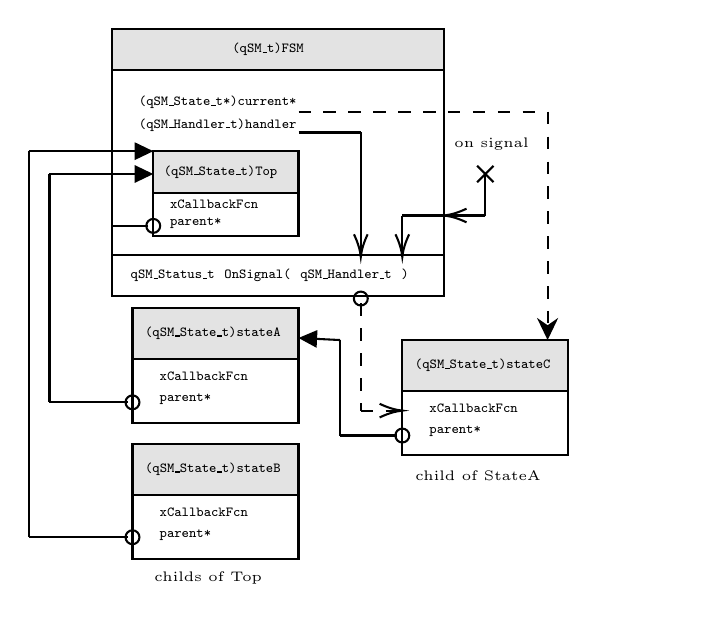
\begin{tikzpicture}[x=0.75pt,y=0.75pt,yscale=-1,xscale=1]
        \draw   (100,40) -- (260,40) -- (260,149) -- (100,149) -- cycle ;
        \draw  [fill={rgb, 255:red, 210; green, 210; blue, 210 }  ,fill opacity=0.62 ] (100,20) -- (260,20) -- (260,40) -- (100,40) -- cycle ;
        \draw   (120,99) -- (190,99) -- (190,120) -- (120,120) -- cycle ;
        \draw  [fill={rgb, 255:red, 210; green, 210; blue, 210 }  ,fill opacity=0.62 ] (120,79) -- (190,79) -- (190,99) -- (120,99) -- cycle ;
        \draw    (60,79) -- (117,79) ;
        \draw [shift={(120,79)}, rotate = 180] [fill=black  ][line width=0.08]  [draw opacity=0] (8.93,-4.29) -- (0,0) -- (8.93,4.29) -- cycle;
        \draw    (60,79) -- (60,265) ;
        \draw   (110,179) -- (190,179) -- (190,210) -- (110,210) -- cycle ;
        \draw  [fill={rgb, 255:red, 210; green, 210; blue, 210 }  ,fill opacity=0.62 ] (110,154.5) -- (190,154.5) -- (190,179) -- (110,179) -- cycle ;
        \draw    (107.65,200) -- (70,200) ;
        \draw [shift={(110,200)}, rotate = 180] [color=black  ][line width=0.75]      (0, 0) circle [x radius= 3.35, y radius= 3.35];
        \draw   (100,129) -- (260,129) -- (260,149) -- (100,149) -- cycle ;
        \draw    (210,170) -- (193,169.15) ;
        \draw [shift={(190,169)}, rotate = 362.86] [fill=black  ][line width=0.08]  [draw opacity=0] (8.93,-4.29) -- (0,0) -- (8.93,4.29) -- cycle    ;
        \draw    (237.65,216) -- (210,216) ;
        \draw [shift={(240,216)}, rotate = 180] [color=black  ][line width=0.75]      (0, 0) circle [x radius= 3.35, y radius= 3.35]   ;
        \draw    (70,90) -- (70,200) ;
        \draw    (70,90) -- (117,90) ;
        \draw [shift={(120,90)}, rotate = 180] [fill=black  ][line width=0.08]  [draw opacity=0] (8.93,-4.29) -- (0,0) -- (8.93,4.29) -- cycle    ;
        \draw    (280,90) -- (280,110) ;
        \draw [shift={(280,90)}, rotate = 135] [color=black  ][line width=0.75]    (-5.59,0) -- (5.59,0)(0,5.59) -- (0,-5.59)   ;
        \draw  [dash pattern={on 4.5pt off 4.5pt}]  (190,60) -- (310,60) ;
        \draw  [dash pattern={on 4.5pt off 4.5pt}]  (310,60) -- (310,167) ;
        \draw [shift={(310,170)}, rotate = 270] [fill=black  ][line width=0.08]  [draw opacity=0] (10.72,-5.15) -- (0,0) -- (10.72,5.15) -- (7.12,0) -- cycle;
        \draw    (280,110) -- (262,110) ;
        \draw [shift={(260,110)}, rotate = 360] [color=black  ][line width=0.75]    (10.93,-3.29) .. controls (6.95,-1.4) and (3.31,-0.3) .. (0,0) .. controls (3.31,0.3) and (6.95,1.4) .. (10.93,3.29)   ;
        \draw    (117.65,115) -- (108.5,115) -- (100,115) ;
        \draw [shift={(120,115)}, rotate = 180] [color=black  ][line width=0.75]      (0, 0) circle [x radius= 3.35, y radius= 3.35]   ;
        \draw    (220,70) -- (220,128) ;
        \draw [shift={(220,130)}, rotate = 270] [color=black  ][line width=0.75]    (10.93,-3.29) .. controls (6.95,-1.4) and (3.31,-0.3) .. (0,0) .. controls (3.31,0.3) and (6.95,1.4) .. (10.93,3.29)   ;
        \draw    (190,70) -- (220,70) ;
        \draw    (210,170) -- (210,216) ;
        \draw  [dash pattern={on 4.5pt off 4.5pt}]  (220,152.35) -- (220,204) ;
        \draw [shift={(220,150)}, rotate = 90] [color=black  ][line width=0.75]      (0, 0) circle [x radius= 3.35, y radius= 3.35]   ;
        \draw  [dash pattern={on 4.5pt off 4.5pt}]  (220,204) -- (238,204) ;
        \draw [shift={(240,204)}, rotate = 180] [color=black  ][line width=0.75]    (10.93,-3.29) .. controls (6.95,-1.4) and (3.31,-0.3) .. (0,0) .. controls (3.31,0.3) and (6.95,1.4) .. (10.93,3.29)   ;
        \draw    (240,110) -- (260,110) ;
        \draw    (240,110) -- (240,128) ;
        \draw [shift={(240,130)}, rotate = 270] [color=black  ][line width=0.75]    (10.93,-3.29) .. controls (6.95,-1.4) and (3.31,-0.3) .. (0,0) .. controls (3.31,0.3) and (6.95,1.4) .. (10.93,3.29)   ;
        \draw    (107.65,265) -- (60,265) ;
        \draw [shift={(110,265)}, rotate = 180] [color=black  ][line width=0.75]      (0, 0) circle [x radius= 3.35, y radius= 3.35]   ;
        \draw   (110,244.5) -- (190,244.5) -- (190,275.5) -- (110,275.5) -- cycle ;
        \draw  [fill={rgb, 255:red, 210; green, 210; blue, 210 }  ,fill opacity=0.62 ] (110,220) -- (190,220) -- (190,244.5) -- (110,244.5) -- cycle ;
        \draw   (240,194.5) -- (320,194.5) -- (320,225.5) -- (240,225.5) -- cycle ;
        \draw  [fill={rgb, 255:red, 210; green, 210; blue, 210 }  ,fill opacity=0.62 ] (240,170) -- (320,170) -- (320,194.5) -- (240,194.5) -- cycle ;
    
        \draw (215,30) node  [font=\ttfamily, text width=3cm] [align=left] {\tiny (qSM\_t)FSM};
        \draw (170,55.5) node  [font=\ttfamily, text width=3cm] [align=left] {\tiny (qSM\_State\_t*)current*};
        \draw (182,89) node  [font=\ttfamily, text width=3cm] [align=left] {\tiny (qSM\_State\_t)Top };
        \draw (185,113.5) node  [font=\ttfamily, text width=3cm] [align=left] {\tiny parent*};
        \draw (173,166.75) node  [font=\ttfamily, text width=3cm] [align=left] {\tiny (qSM\_State\_t)stateA};
        \draw (185,139) node  [font=\ttfamily, text width=4cm] [align=left] {\tiny qSM\_Status\_t OnSignal( qSM\_Handler\_t )};
        \draw (276.5,235.5) node  [font=\tiny] [align=left] {child of StateA};
        \draw (185,104.5) node  [font=\ttfamily, text width=3cm] [align=left] {\tiny xCallbackFcn};
        \draw (180,198.5) node [font=\ttfamily, text width=3cm] [align=left] {\tiny parent*};
        \draw (180,187.5) node  [font=\ttfamily, text width=3cm] [align=left] {\tiny xCallbackFcn};
        \draw (170,66.5) node  [font=\ttfamily, text width=3cm] [align=left] {\tiny (qSM\_Handler\_t)handler};
        \draw (283,75.5) node  [font=\tiny] [align=left] {on signal};
        \draw (173,232.25) node  [font=\ttfamily, text width=3cm] [align=left] {\tiny (qSM\_State\_t)stateB};
        \draw (180,264) node   [font=\ttfamily, text width=3cm] [align=left] {\tiny parent*};
        \draw (180,253) node  [font=\ttfamily, text width=3cm] [align=left] {\tiny xCallbackFcn};
        \draw (146.5,284.5) node  [font=\tiny] [align=left] {childs of Top};
        \draw (303,182.25) node  [font=\ttfamily, text width=3cm] [align=left] {\tiny (qSM\_State\_t)stateC};
        \draw (310,214) node  [font=\ttfamily, text width=3cm] [align=left] {\tiny parent*};
        \draw (310,203) node  [font=\ttfamily, text width=3cm] [align=left] {\tiny xCallbackFcn};
    \end{tikzpicture}
    \caption{FSM module design}
    \label{fig:fsmdesign}
\end{figure}